\documentclass[article,table]{aaltoseries}
\usepackage[utf8]{inputenc}
\usepackage{url}
\usepackage{multirow}

\begin{document}
 
%=========================================================

\title{Digital Twins for Industrial Edge 4.0: Concepts and Tools}

\author{Adika Bintang Sulaeman% Your first and last name: do _not_ add your student number
\\\textnormal{\texttt{adika.sulaeman@aalto.fi}}} % Your Aalto e-mail address

\affiliation{\textbf{Tutor}: Prof. Hong-Linh Truong} % First and last name of your tutor

\maketitle

%==========================================================

\begin{abstract}
  Industry 4.0 is expected to be the next big phase in industry. Digital Twins (DT), defined as digital representations of physical objects such as machines, have an important role in Industry 4.0. This seminar paper discusses an overview of DT technology, key technologies to implement DT, DT frameworks, DT tools and how they can be combined to build DT systems. From the literature study conducted, the existing works from previous research can be combined to build DT systems.
  
\vspace{3mm}
\noindent KEYWORDS: Digital Twins, Industry 4.0, Frameworks, Tools

\end{abstract}


%============================================================


\section{Introduction}

Industry 4.0 is the next big phase in industry. With Industry 4.0, it is possible to gather real-time data from the machines that run in industry and process the data into something meaningful and useful. Industry 4.0 mainly consists of three supporting technologies: IoT, Cyber-Physical Systems (CPS), and Smart Factories \cite{hermann2016design}. The combination of these technologies builds interconnected devices forming Digital Twins (DT).

A DT models a physical object by creating a digital representation using real-time data \cite{Cheatshe3:online}. The data is gathered throughout its life-cycle and used as the source to monitor, learn from, and enhance decision making. A DT enables engineers to monitor and understand how the machines behave once it is released and run by users. Furthermore, engineers can analyze the data and predict the future performance of the machines.

There are some use cases of DT for Industry 4.0. Consider a Printed Circuit Board (PCB) printer for electronic manufacturers. The PCB printer must be very precise, because the smallest error by the laser cutter may lead to PCB flaws. A DT enables engineers and technicians to monitor and analyze the data to predict the time when the spare parts wear out. Another example would be monitoring the jet engine of airplanes. By analyzing data gathered in real-time, engineers and technicians may predict failures in jet systems, which will lead to the reduction of airplane incidents. Furthermore, DT may give feedback to the engineers who design the machine to help them realize an agile development system.

The main value that the DT delivers is an understanding of product performance \cite{Cheatshe3:online}. By understanding performance, manufacturers may detect and understand faults better, create an effective maintenance schedule, troubleshoot machines remotely, and decide appropriate add-on services.

The DT has some challenges in its development and implementation. In \cite{bienhaus2017patterns}, the author has stated a number of challenges such as data consistency between the real physical assets and the digital representation, as well as connectivity and security concerns of cloud computing for DT. Software architectural aspects such as internal structure, APIs, integration, and runtime environment are also critical challenges for DT \cite{malakuti2018architectural}.

\subsection{Scope and Goals}
\label{sec:emphasis}
This paper aims to review the concept of DT for manufacturing in Industry 4.0 as well as technologies to build the DT system. This seminar paper is intended as a review paper for DT developers to build DT systems.

\subsection{Structure}
\label{sec:em}
The rest of this paper is organized as follows. Section 2 discusses the key technologies for DT. Section 3 discusses the existing DT framework approaches and tools to build the DT framework. Section 4 concludes this review paper.
 

%============================================================



%============================================================

\section{Principles of Building Digital Twin Systems}
\subsection{Requirement Analysis of Digital Twin Systems}
There are for requirements for building DT systems \cite{Tao2019}. These requirements can be used to determine key technologies for building DT systems.

From the aspect of DT applications, the first requirement is DT systems must be general enough to support various applications such as manufacturing, construction, and health-care.

From the technologies aspect, since the main aim of the DT is to fuse the interaction in CPS, the DT must embrace the integration of new generation information technologies such as IoT, cloud computing, big data, and artificial intelligence (AI) to support its goal.

From the modeling object aspect, the DT must integrate and fuse operational data from physical space and simulated data from virtual space. The DT must also be encapsulated as services which have user-friendly interface and ease the user operations.

From the modeling method aspect, the DT requires high-fidelity virtual modeling. The virtual modeling includes geometrical, physical, behavior, and rules modeling.

\subsection{Key Technologies of Digital Twins}
The requirements analysis leads to the abstraction of the DT concept model. Fig.~\ref{fig:Tao_DT_concept_model} shows the DT concept model which is divided into five dimensions, i.e., the Physical Entity (PE), Virtual Entity (VE), Services (Ss), DT Data (DD) and Connection (CN). Each of these components has its own key technologies to build the DT system as a whole as shown in Fig.~\ref{fig:Tao_DT_key_techs} \cite{Tao2019}.

\begin{figure}[t!]
	\begin{center}
		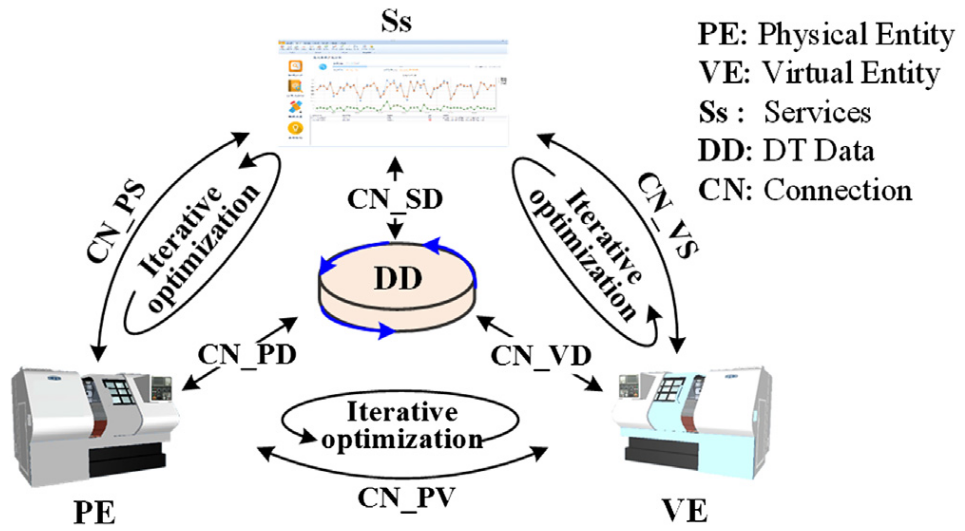
\includegraphics[width=1\textwidth]{figures/Tao_DT_concept_model}
		\caption{DT concept model \cite{Tao2019}}
		\label{fig:Tao_DT_concept_model}
	\end{center}
\end{figure}

\begin{figure}[t!]
	\begin{center}
		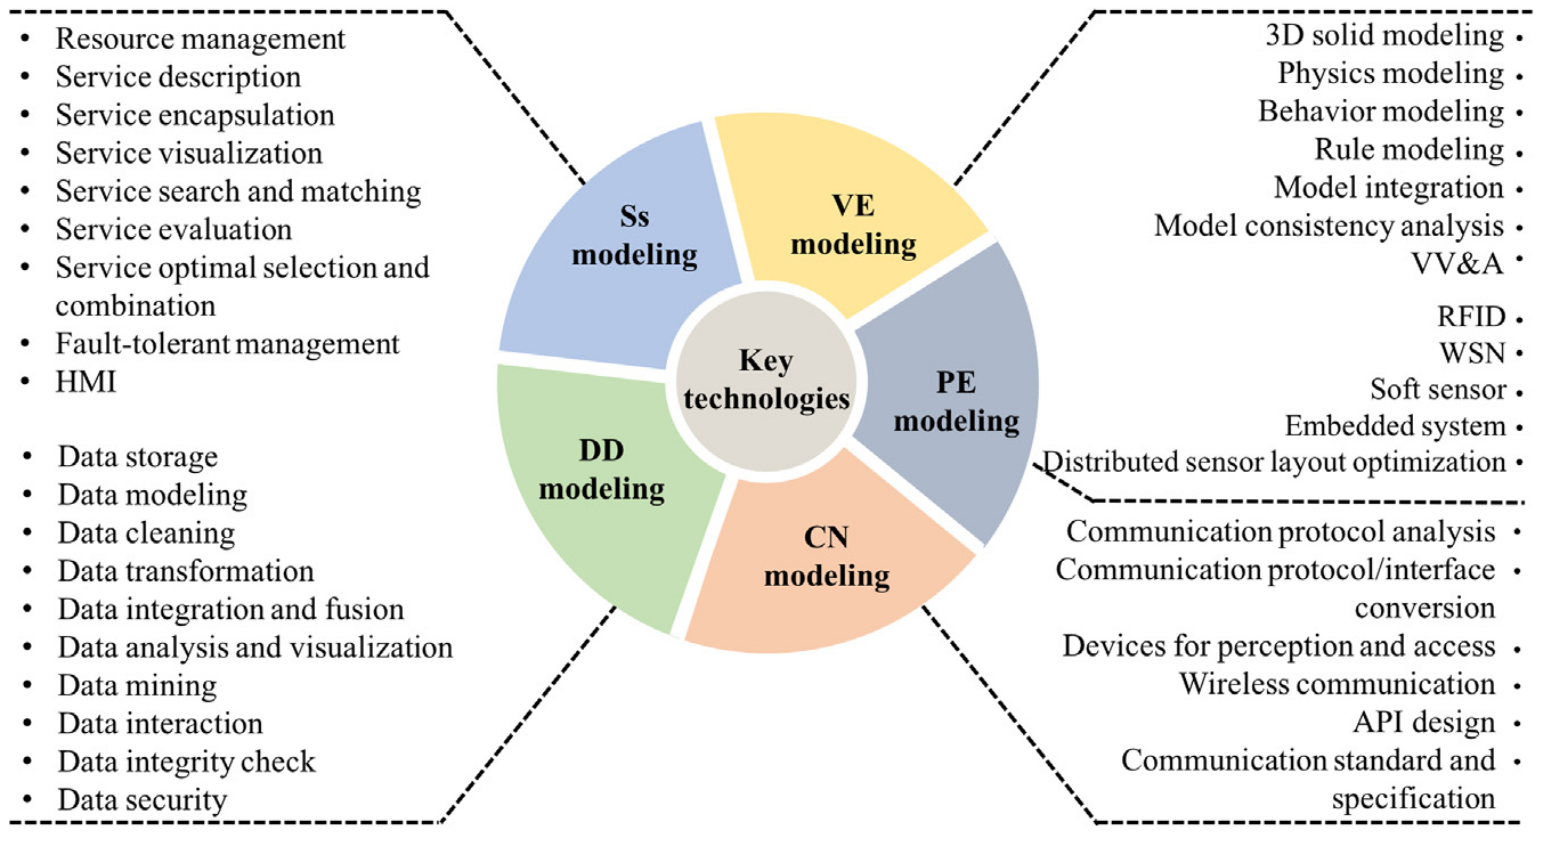
\includegraphics[width=1\textwidth]{figures/Tao_DT_key_techs}
		\caption{Key technologies for DT \cite{Tao2019}}
		\label{fig:Tao_DT_key_techs}
	\end{center}
\end{figure}

The PE is the real physical entity in the physical space. It contains the real machines with their sensors and actuators. The technologies in the PE includes embedded systems to embed computing capabilities to the entities, RFID to track and identify the entities, Wireless Sensor Network (WSN) to transmit sensors' data and distributed sensor layout optimization to reduce information redundancy.

The VE consists of a set of models representing the PE. Modeling techniques such as three-dimension solid modeling, physics modeling, behavior modeling, and rule modeling are needed to create useful modeling of the PE. To keep PE and VE model consistent, model consistency analysis, verification, validation and accreditation must be implemented.

The Ss of the DT serves other DT dimensions' needs. The services used by PE include monitoring service, state prediction service, and energy consumption optimization service. VE uses the construction service, calibration service and test service for modeling. Some aspects are needed to create and maintain Ss, i.e., resource management, service description, service encapsulation, service visualization, service search and matching, service evaluation, service optimal selection and combination, fault-tolerant management and human-machine interface (HMI).

The DD contains data from physical and virtual space. Therefore, the number of heterogeneous data is high. Technologies for processing and securing data, such as data storage, data modeling, data transformation, data cleaning, data analysis, data mining, data integrity check and data security, are required in helping modeling DT data.

The CN connects different elements of DT. It enables PE, VE, Ss, and DD to communicate with each other. Key technologies of CN includes communication protocol analysis, communication protocol/interface conversion, wireless communication, Application Programming Interface (API) design, as well as communication standard and specification.

\section{Implementing Digital Twin Systems}
This section starts by discussing the existing DT frameworks, which give guideline or supporting structures for building DT systems. Then, it continues to discuss tools to realize DT framework. Finally, the discussion of the combination of DT frameworks and tools is presented.

\subsection{Digital Twin Frameworks}
Some researchers have proposed frameworks for building DT. While some of them propose holistic frameworks, there are also frameworks focusing on one particular part of DT. Table~\ref{tab:table_tools} shows a brief summary of the discussed frameworks.

\begin{table}[]
	\begin{tabular}{|l|p{4.5cm}|p{7.3cm}|}
		\hline
		\rowcolor[HTML]{C0C0C0} 
		Framework                                                                    & Focus                                                                                 & Future works (not implemented yet)                                                                                                                                                                                                                                  \\ \hline
		Zheng et al. \cite{zheng2019application}                                                         & Application framework for DT in manufacturing                                         & Data synchronization; mapping methods between physical and digital space; application mode of DT                                                                                                                                                                    \\ \hline
		Zhuang et al. \cite{Zhuang2018}                                                                   & Framework of DT-based smart production management and control for assembly shop-floor & Construction and optimization of IoT networks in a physical assembly shop floor; construction, optimization, and running of an assembly shop-floor DT; construction of big data management platform; modeling and implementation of smart decision making algorithm \\ \hline
		Zhang et al. \cite{Zhang2017}                                                                    & DT modeling based on perception data modeled as ontology                              & Dynamic linkage between physical, digital, 3D; fully functional service system; AR for 3D models                                                                                                                                                                    \\ \hline
		Qi et al. \cite{qi2018modeling}                                                               & Combining edge, fog, and cloud to build DT system                                     & Increase the number of and the capbilities of edge nodes; architecture, platform, and standard of fog computing; data filtering to choose which data to process in edge, fog, and cloud; energy consumption; security                                               \\ \hline
		Lynn et al. \cite{lynn2018realization}                                                          & modeling and controling physical space through DT                                     & Automated plan generation; enhanced trajectory planning                                                                                                                                                                                                             \\ \hline
		Botkina et al. \cite{botkina2018digital}                                                           & modeling and controling physical space through DT                                     & Integrating non-tweeting machines to the system                                                                                                                                                                                                                     \\ \hline
		Ciavotta et al. \cite{ciavotta2017microservice} & Software service for DT based on microservice                                         & IoT protocols such as MQTT for CPS communication; AutomationML for data exchange                                                                                                                                                                                    \\ \hline
	\end{tabular}
	\caption{Existing DT frameworks}
	\label{tab:framework_tools}
\end{table}

Two examples of holistic frameworks for building DT were proposed by Yu Zheng et al. \cite{zheng2019application} and Zhuang et al. \cite{Zhuang2018}. The framework proposed by Yu Zheng et al. aims to realize full-physical system mapping, life-cycle dynamic modeling, and the whole process of real-time optimization. The framework proposed by Zhuang et al. aims to build DT-based smart production management and control framework for product assembly shop-floor.

Although both frameworks were proposed to build DT for manufacturing, they have different approaches. The framework proposed by Yu Zheng et al. divided the system into three dimensions, i.e, physical space, virtual space, and information-processing layer. On the other hand, the framework proposed by Zhuang et al. divided the system into four dimensions, i.e., management of the physical space, construction of the virtual space of the shop-floor, DT and big-data driven prediction and production management and control service of the assembly shop-floor.

Zhang et al. proposed another framework focusing on modeling DT workshop based on perception data \cite{Zhang2017}. The framework consists of three parts, i.e., physical model, ontology-based digital model, and the virtual model. The ontology-based data modeling is what makes this framework different from the others.

The aforementioned frameworks are the examples of the complete DT framework, starting from the physical to the virtual entity. However, they do not thoroughly describe the frameworks for each of the specific DT dimensions.

The service dimension of DT mentioned in section 2 is crucial for DT system because it connects one dimension to the others. There are many ways to build software services.

Ciavotta et al. suggested the use of microservice architecture for building middleware as a service for DT \cite{ciavotta2017microservice}. This middleware supports data collecting, authentication, and accessing DT resource and data. The benefits of using microservice architecture include agility, isolation, and resilience as well as elasticity. However, it also increases the system complexity at the same time.

The PE dimension of DT may come with different messaging formats and protocols. Software service middleware must support a variety of data formats coming from different dimensions of DT. For example, Schroeder et al. proposed a framework for building middleware to accept AutomationML data format and convert them into other data format via REST API \cite{Schroeder2016automationml}.

Several frameworks for virtual entity have also been proposed. Schroeder et al. proposed the use of Augmented Reality (AR) to visualize DT \cite{schroeder2016visualising}, leveraging Vuforia Engine to build the AR system. For controlling physical devices through DT in VE, Lynn et al. \cite{lynn2018realization} and Botkina et al. \cite{botkina2018digital} have slightly different approaches. The framework proposed by Lynn et al. used raw TCP for controlling the device and raw UDP for getting the feedback data from the device, whereas the Botkina et al. approach used the standard Line Information System Architecture (LISA) and ISO 13399.

So far, all the frameworks discussed suggest the use of cloud computing for their processing and storage. However, some applications are latency sensitive. Bringing data to the cloud which can be physically far from the source of data may add significant latency overhead.

Qi Zhang et al. proposed a DT framework based on edge computing, fog computing and cloud computing to improve efficiency and reduce latency \cite{qi2018modeling}. In many cases, the data processing and control of physical objects require very low latency. Therefore, edge computing architecture resides on the unit level to achieve that goal. The unit level entities are connected to the information management systems such as Enterprise Resource Planning (ERP) and Manufacturing Execution System (MES). Fog computing is suitable for connecting CPS to DT to improve efficiency. Finally, the data can also be stored and processed in the cloud at the SoS level for various purposes such as data analysis and long-term storage.

\subsection{Tools for Digital Twins}
In this subsection, tools or sets of software which equip the DT frameworks are discussed. 

The PE needs tools to control, sample the operation and environment data, as well as send them to other dimensions of DT. MachineKit is an open-source platform for controlling machines, enabling users to control servo motors of Computer Numerical Control (CNC) machine based on the commands sent by VE \cite{lynn2018realization}.

The CN dimension, which connects PE to other dimensions of DT, represents the IoT in general. While there are many protocols and communication mechanisms for IoT, not all of them fits into industrial applications. OPC Unified Architecture (OPC UA) is a machine-to-machine communication protocol that is used by the framework proposed by Yu Zheng et al. \cite{zheng2019application}. MTConnect is another mechanism to retrieve data from machine tools. Coronado et al. used MTConnect to retrieve the data from the physical space to their DT system \cite{UrbinaCoronado2018}.

MES software is commonly used for both collecting data and monitor process and operation of the manufacturing process. MES is generally proprietary and expensive. As a result, small manufacturing enterprise may have difficulties in deploying MES in their system.

Coronado  came up with a low-cost MES system based on Android \cite{UrbinaCoronado2018}. This tool captures part and tooling information using an Android-based MES. The data from MES is combined with data from device sensors to represent parts, operators, capital equipment and consumable in shop-floor DT. This tool supports the Ss dimension of DT as an HMI and resource management tool.

There are various supporting tools for building the DT services, depending on the system architecture of the service. FIWARE is a middleware for exhanging data that can be used as a service for DT \cite{Schroeder2016automationml}. MAYA Support Infrastructure middleware used Netflix Eureka for service discovery and Elasticsearch-Logstash-Kibana (ELK) for log monitoring \cite{ciavotta2017microservice}. The recent trend in microservice technology is to scale the service horizontally; leveraging containers to deploy the services. For this case, containers orchestration tools such as Docker Swarm and Kubernetes may support the system. However, the containerization is not a silver bullet solution since it may impact the network performance in transfer rate and packet loss negatively \cite{kratzke2017microservices}.

The data from both physical space and virtual space must be stored in a database system. Depending on how the data is structured, several options for database platforms are available. For structured data, ODBC-compliant database such as MySQL can be used to store the data \cite{Zhang2017}. For unstructured data, NoSQL platform such as Apache Cassandra can be used \cite{ciavotta2017microservice}.

There are some tools, open source or proprietary, available to support the DT framework in VE dimension. To control machine tools from the VE, Computer-Aided Manufacturing (CAM) software such as SculptPrint can be used \cite{lynn2018realization}. Vuforia Engine can be used to leverage AR technology in building the VE \cite{schroeder2016visualising}. To build 3D models of the physical objects, SolidWorks, Pro/E and CATIA can be used \cite{Zhuang2018}. FlexSim can be used as a software simulation for manufacturing process \cite{Zhang2017}. Table~\ref{tab:table_tools} summarizes the tools for building DT systems.

% Please add the following required packages to your document preamble:
% \usepackage{multirow}
% \usepackage[table,xcdraw]{xcolor}
% If you use beamer only pass "xcolor=table" option, i.e. \documentclass[xcolor=table]{beamer}
\begin{table}[]
	\begin{tabular}{|p{3.8cm}|p{1.5cm}|p{5.8cm}|}
		\hline
		\rowcolor[HTML]{C0C0C0} 
		Tools                                                        & Domain & Roles                                                                                   \\ \hline
		MachineKit                                                   & PE             & Platform for machine control applications                                               \\ \hline
		MTConnect                                                    & CN             & Manufacturing standard to retrieve information from machines                            \\ \hline
		OPC UA                                                       & CN             & Machine to machine communication for industrial automation                              \\ \hline
		FIWARE                                                       & Ss             & Middleware for data exchange                                                            \\ \hline
		Netflix Eureka                                               & Ss             & Service discovery in microservice architecture                                          \\ \hline
		Docker/containerd and Docker swarm/Kubernetes                & Ss             & Containerization and orchestration of deployed services                                 \\ \hline
		Relational data storage (MySQL, PostgreSQL)                  & DD             & SQL database                                                                            \\ \hline
		NoSQL data storage (Apache Cassandra)                        & DD             & NoSQL database                                                                          \\ \hline
		FlexSim                                                      & VE             & Simulation software to model, simulate, predict, and visualize systems in manufacturing \\ \hline
		SculptPrint                                                  & VE             & Software for generating tool paths for 5-axis machine tools                             \\ \hline
		CATIA                                                        & VE             &                                                                                         \\ \cline{1-2}
		SolidWorks                                                   & VE             &                                                                                         \\ \cline{1-2}
		Pro/E                                                        & VE             & \multirow{-3}{*}{3D physical modeling}                                                  \\ \hline
		Android-based MES \cite{UrbinaCoronado2018} & Ss and VE      & Low cost and open source based Manufacturing Execution System (MES)                     \\ \hline
	\end{tabular}
	\caption{Tools for building DT systems}
	\label{tab:table_tools}
\end{table}

\subsection{Discussion}
Several DT frameworks have been discussed to analyze the use cases and limitations. From the limitations and future works of those frameworks, a more complete framework can be built. In principle, the new framework can be formed by combining existing frameworks and adjusted to the application requirements.

For controlling machines in physical space, the framework proposed by Botkina et al. \cite{botkina2018digital} must have tweeting machines in the shop-floor. While this tweeting machines development is not discussed, Lynn et al. \cite{lynn2018realization} describe the mechanism of sending feedback data from actuators with raw UDP. The use of raw UDP by Lynn et al. might not be applicable if it does not comply with existing standards. Instead, OPC UA can be used as the protocol, as the framework developed by Yu Zheng et al. used \cite{zheng2019application}.

The services in DT is described by the framework proposed by Ciavotta et al. \cite{ciavotta2017microservice}. This service is supposed to be deployed in the cloud. However, it does not cover the latency sensitive applications. The combination of the framework proposed by Ciavotta et al. and Qi et al. \cite{qi2018modeling} might be the solution for case sensitive applications since it offers the use of edge, fog, and cloud computing to deploy the services. Furthermore, the use of containers and orchestration in fog, edge, and cloud computing might be used to ease the deployment, maintenance and horizontal scaling of the services. 

For modeling the physical space in the virtual space, framework proposed by Zhuang et al. \cite{Zhuang2018} covers the data flow, Zhang et al. \cite{Zhang2017} proposed the use of ontology for modeling the data, and Schroeder et al. \cite{schroeder2016visualising} proposed the use of AR to model the physical space in VE domains. The combinations of these three modeling frameworks might be useful to create a robust, complete, and useful mechanism of modeling DT systems.

In conclusion, the fusion of these frameworks can be combined according to the application requirements, cost and available resources. 

\section{Conclusion and Future Work}
DT represents physical objects such as industrial machines as digital entities. DT can help monitoring machines and understanding product performance.

DT can conceptually be divided into five dimensions, i.e., the Physical Entity (PE), Virtual Entity (VE), Services (Ss), DT Data (DD) and Connection (CN). This seminar provides a review of existing frameworks and tools, as well as how they correlate to the aforementioned DT dimensions.

Seven frameworks have been analyzed and their chosen tools for DT are also mentioned. These frameworks and tools can be combined to form a more complete framework or to create a framework specific to some certain application requirements. The tools needed to build the DT system to support the frameworks are also discussed. The key technologies used by these frameworks and tools include IoT, embedded systems, software services and APIs, data storage and processing as well as modeling and controlling software.

The research directions or future work for this DT frameworks and tools include the standardization of connection between physical to digital space, adaptive service for modeling different data format, benchmarking and analyzing existing protocols and message formats as well as latency impact of DT to the control systems.

 

%============================================================

\bibliographystyle{plain}
\bibliography{cs-seminar}

\end{document}
